\chapter{Generator Avatar dengan Elixir: Bagian 1}

\section{Pendahuluan}
Pada bab ini, akan dibahas pengembangan generator avatar menggunakan bahasa pemrograman Elixir. Kode ini memanfaatkan konsep inti Elixir seperti \texttt{defstruct} untuk mendefinisikan struktur data khusus, \texttt{defmodule} untuk membuat modul, serta menggunakan \texttt{Application} behavior untuk mengelola siklus hidup aplikasi. Generator avatar ini menerima sebuah input, menghitung hash, memilih warna, dan menghasilkan representasi grid dari avatar. Bagian-bagian berikut akan membahas setiap bagian kode secara lebih rinci.

\subsection{Avatar Generator}
\begin{figure}[h]
	\begin{center}
		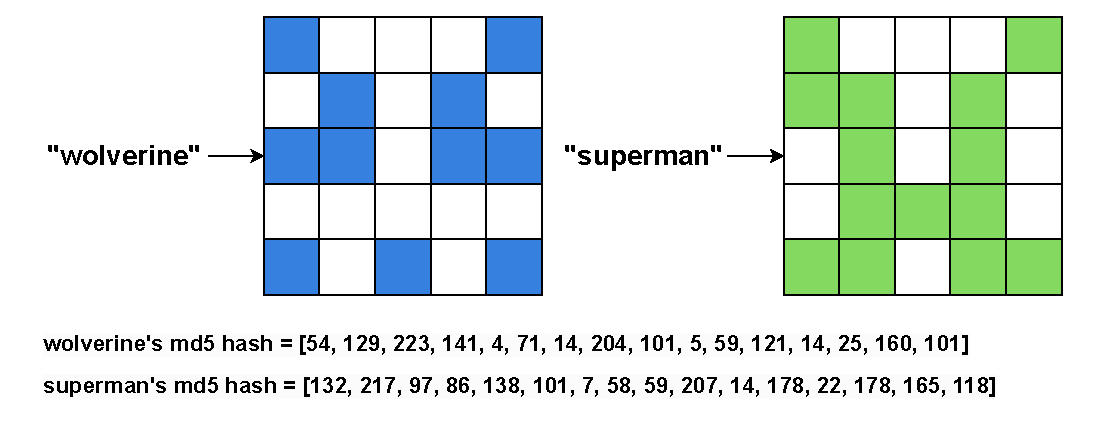
\includegraphics[width=1\textwidth]{../assets/avatar-example.pdf}
	\end{center}
	\caption{Contoh output avatar yang dihasilkan dari username ``wolverine" dan ``superman".}
\end{figure}
	
Pada program generator avatar ini, kata-kata seperti \texttt{"wolverine"} dan \texttt{"superman"} akan diolah dengan menghitung nilai hash-nya menggunakan algoritma MD5. Hash yang dihasilkan berupa daftar angka yang mewakili nilai-nilai biner dari hasil hash tersebut.

Sebagai contoh:
\begin{itemize}
	\item Kata \texttt{"wolverine"} memiliki hash MD5 yang direpresentasikan sebagai daftar angka: 
	\[
	[54, 129, 223, 141, 4, 71, 14, 204, 101, 5, 59, 121, 14, 25, 160, 101]
	\]
	\item Kata \texttt{"superman"} menghasilkan hash MD5 yang direpresentasikan sebagai daftar angka:
	\[
	[132, 217, 97, 86, 138, 101, 7, 58, 59, 207, 14, 178, 22, 178, 165, 118]
	\]
\end{itemize}

Hash ini kemudian digunakan untuk membentuk representasi grid dari avatar. Setiap nilai dalam hash akan digunakan untuk menentukan pola atau warna dari avatar yang dihasilkan, sehingga setiap kata input yang berbeda akan menghasilkan avatar yang unik.


\subsection{Avatar Pipeline}
\begin{figure}[h]
	\begin{center}
		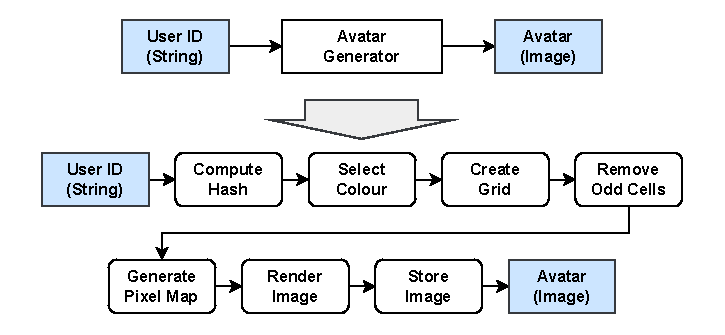
\includegraphics[width=1\textwidth]{../assets/avatar-pipeline.pdf}
	\end{center}
\caption{Rincian \textit{pipeline} dari Avatar Generator.}
\end{figure}

Pipeline pada \texttt{Avatar Generator} terdiri dari urutan pemanggilan fungsi yang digunakan untuk membangkitkan sebuah avatar berdasarkan \texttt{input} yang diberikan. Proses ini dimulai dari fungsi \texttt{compute\_hash}, di mana nilai hash dari \texttt{input} dihitung untuk digunakan pada proses berikutnya. Selanjutnya, fungsi \texttt{select\_color} memilih warna utama yang akan digunakan dalam avatar berdasarkan nilai hash tersebut.

Setelah warna dipilih, fungsi \texttt{create\_grid} akan membuat sebuah grid atau tata letak dari pola-pola avatar yang dihasilkan. Grid ini kemudian akan disaring oleh fungsi \texttt{remove\_odd\_cells} yang menghapus sel-sel ganjil (sel yang tidak sesuai dengan pola tertentu), sehingga menghasilkan tata letak grid yang lebih terstruktur.

Proses selanjutnya adalah menggunakan fungsi \texttt{generate\_pixel\_map} untuk menghasilkan koordinat-koordinat piksel dari sel-sel pada grid yang telah disaring. Fungsi ini akan membuat peta piksel yang menunjukkan posisi dan ukuran masing-masing piksel pada gambar.

Setelah peta piksel terbentuk, fungsi \texttt{render\_image} akan menggambar gambar avatar sesuai dengan warna dan posisi piksel yang telah ditentukan. Hasil gambar tersebut kemudian akan disimpan menggunakan fungsi \texttt{store\_image}, yang menyimpan file avatar dalam format \texttt{PNG} dengan nama file sesuai dengan \texttt{input} yang diberikan.

Dengan demikian, pipeline pada \texttt{Avatar Generator} adalah sebagai berikut:

\begin{lstlisting}[language=Elixir]
	compute_hash
	|> select_color
	|> create_grid
	|> remove_odd_cells
	|> generate_pixel_map
	|> render_image
	|> store_image
\end{lstlisting}

Setiap fungsi dalam pipeline ini memiliki perannya masing-masing dan dihubungkan dengan operator \texttt{|>} untuk mempermudah alur data dari satu fungsi ke fungsi lainnya, sehingga proses pembuatan avatar dapat dilakukan secara berurutan dan terstruktur.

\subsection{Avatar Computation}
\begin{figure}
	\begin{center}		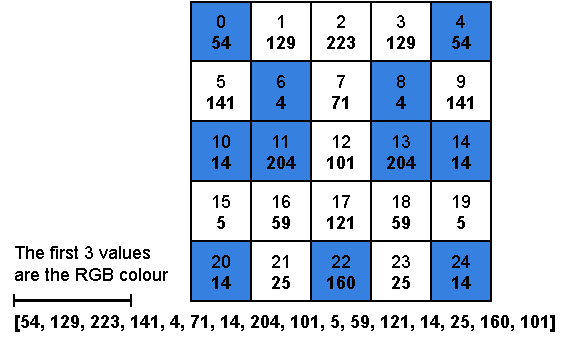
\includegraphics[width=1\textwidth]{../assets/avatar-computation.pdf}
	\end{center}
\caption{Contoh pencerminan dan juga nilai-nilai integer dari hash serta nilai RGB untuk warna.}
\end{figure}

Avatar yang dihasilkan merupakan sebuah file gambar yang terdiri dari 5 baris dan 5 kolom. Struktur kolom dalam avatar ini memiliki pola tertentu, di mana kolom ke-4 merupakan cerminan dari kolom ke-2, dan kolom ke-5 merupakan cerminan dari kolom ke-1. Dengan demikian, pola simetri ini memberikan kesan keseimbangan visual pada avatar yang dihasilkan.

Tiga kolom pertama dari kelima baris tersebut diisi dengan nilai-nilai yang diambil dari hash MD5 dari \texttt{username}. Dalam pengisian kolom-kolom ini, nilai-nilai yang genap akan diwarnai sesuai dengan ketentuan yang telah ditentukan, sementara nilai-nilai ganjil akan dibiarkan berwarna putih. 

Selanjutnya, tiga nilai pertama dari hash MD5 akan digunakan sebagai warna RGB untuk mengisi sel-sel yang bernilai genap. Dengan demikian, avatar tidak hanya terstruktur secara geometris, tetapi juga memiliki elemen warna yang ditentukan oleh karakteristik unik dari \texttt{username} yang di-hash. Proses ini menghasilkan sebuah gambar avatar yang menarik dan personal, mencerminkan identitas pengguna secara visual.

\section{Keseluruhan Kode}

\begin{lstlisting}[language=Elixir, caption={Keseluruhan Kode src/avatar.ex}]
defmodule AvatarGenerator do
use Application

def generate(input) do
input
|> compute_hash
|> select_color
|> create_grid
end

@spec create_grid(%Avatar.Image{:hash => any(), optional(any()) => any()}) :: [
{any(), integer()}
]
def create_grid(%Avatar.Image{hash: hash} = image) do
hash
|> Enum.chunk_every(3)
|> Enum.map(&reflect_row/1)
|> List.flatten
|> Enum.with_index
end

def reflect_row(row) do
[ first, second | _tail] = row
row ++ [second, first]
end

def compute_hash(input) do
hash =
:crypto.hash(:md5, input)
|> :binary.bin_to_list()
|> resize_list

IO.inspect(hash)
%Avatar.Image{hash: hash}
end

def resize_list(list) do
full_chunks_count = div(length(list), 3) * 3
Enum.take(list, full_chunks_count)
end

def select_color(%Avatar.Image{hash: [r, g, b | _tail]} = image) do
%Avatar.Image{image | color: {r, g, b}}
end

def start(_type, _args) do
result = AvatarGenerator.generate("wolverine")
IO.inspect(result)
{:ok, self()}
end
end

\end{lstlisting}

\begin{lstlisting}[language=Elixir, caption={Keseluruhan Kode src/image.ex}]
defmodule Avatar.Image do
	defstruct hash: nil, color: nil
end
\end{lstlisting}

\section{Struktur Modul}
Program ini terdiri dari dua modul:

\begin{itemize}
	\item \textbf{Avatar.Image}: Modul yang mendefinisikan struktur untuk menyimpan informasi terkait avatar seperti hash dan warna.
	\item \textbf{AvatarGenerator}: Modul utama yang bertanggung jawab untuk menghasilkan avatar dengan menghitung hash, memilih warna, dan membuat grid.
\end{itemize}

\subsection{Mendefinisikan Struktur Avatar Image}
Modul \texttt{Avatar.Image} mendefinisikan struktur yang akan digunakan untuk menyimpan informasi hash dan warna dari avatar. Struktur ini didefinisikan menggunakan kata kunci \texttt{defstruct}.

\begin{lstlisting}[language=Elixir, caption={Mendefinisikan struktur Avatar Image di \texttt{lib/image.ex}}]
	defmodule Avatar.Image do
	defstruct hash: nil, color: nil
	end
\end{lstlisting}

Kata kunci \texttt{defstruct} digunakan untuk mendefinisikan struktur dengan atribut \texttt{hash} dan \texttt{color}. Atribut-atribut ini awalnya diatur menjadi \texttt{nil} dan akan diisi seiring dengan proses pembuatan avatar.

\subsection{Modul Generator Avatar}
Modul \texttt{AvatarGenerator} adalah modul inti yang menangani logika pembuatan avatar. Modul ini menggunakan \texttt{Application} behavior, yang memungkinkan untuk mendefinisikan fungsi \texttt{start/2} guna menginisialisasi aplikasi.

\begin{lstlisting}[language=Elixir, caption={Definisi modul Avatar Generator di \texttt{lib/avatar.ex}}]
	defmodule AvatarGenerator do
	use Application
\end{lstlisting}

\subsection{Pembuatan Avatar}
Fungsi \texttt{generate/1} adalah fungsi utama yang menangani pembuatan avatar. Fungsi ini menerima sebuah string \texttt{input}, menghitung hash, memilih warna, dan membuat representasi grid dari avatar.

\begin{lstlisting}[language=Elixir, caption={Fungsi utama untuk pembuatan avatar}]
	def generate(input) do
	input
	|> compute_hash
	|> select_color
	|> create_grid
	end
\end{lstlisting}

Fungsi \texttt{generate/1} menggunakan operator pipa (\texttt{|>}) untuk meneruskan hasil dari setiap fungsi ke fungsi berikutnya dalam pipeline. Ini memastikan alur kode yang bersih dan mudah dibaca.

\subsection{Menghitung Hash}
Fungsi \texttt{compute\_hash/1} menggunakan modul \texttt{:crypto} untuk menghasilkan hash MD5 dari string input. Hash biner yang dihasilkan kemudian dikonversi menjadi daftar integer dan diubah ukurannya agar panjangnya menjadi kelipatan tiga.

\begin{lstlisting}[language=Elixir, caption={Menghitung hash dari string input}]
	def compute_hash(input) do
	hash =
	:crypto.hash(:md5, input)
	|> :binary.bin_to_list()
	|> resize_list
	
	IO.inspect(hash)
	%Avatar.Image{hash: hash}
	end
\end{lstlisting}

Fungsi pembantu \texttt{resize\_list/1} digunakan untuk memastikan bahwa panjang daftar hash adalah kelipatan 3. Hal ini diperlukan untuk membuat representasi grid avatar yang simetris.

\begin{lstlisting}[language=Elixir, caption={Mengubah ukuran daftar hash}]
	def resize_list(list) do
	full_chunks_count = div(length(list), 3) * 3
	Enum.take(list, full_chunks_count)
	end
\end{lstlisting}

\subsection{Memilih Warna Avatar}
Fungsi \texttt{select\_color/1} mengekstrak tiga elemen pertama dari daftar hash dan menggunakannya untuk mendefinisikan nilai RGB dari warna avatar.

\begin{lstlisting}[language=Elixir, caption={Memilih warna avatar dari hash}]
	def select_color(%Avatar.Image{hash: [r, g, b | _tail]} = image) do
	%Avatar.Image{image | color: {r, g, b}}
	end
\end{lstlisting}

Warna direpresentasikan sebagai tuple \texttt{\{r, g, b\}}, di mana \texttt{r}, \texttt{g}, dan \texttt{b} masing-masing adalah komponen merah, hijau, dan biru dari warna tersebut.

\subsection{Membuat Grid Avatar}
Fungsi \texttt{create\_grid/1} mengubah hash menjadi pola grid dengan memecah daftar hash menjadi baris-baris yang masing-masing terdiri dari tiga elemen, kemudian mencerminkan setiap baris untuk menciptakan simetri. Baris-baris ini kemudian dipipihkan dan diberi indeks.

\begin{lstlisting}[language=Elixir, caption={Membuat grid avatar}]
	def create_grid(%Avatar.Image{hash: hash} = image) do
	hash
	|> Enum.chunk_every(3)
	|> Enum.map(&reflect_row/1)
	|> List.flatten
	|> Enum.with_index
	end
\end{lstlisting}

Fungsi pembantu \texttt{reflect\_row/1} menduplikasi dua elemen pertama dari setiap baris dalam urutan terbalik, memastikan bahwa grid yang dihasilkan adalah simetris.

\begin{lstlisting}[language=Elixir, caption={Mencerminkan baris untuk menciptakan simetri}]
	def reflect_row(row) do
	[ first, second | _tail] = row
	row ++ [second, first]
	end
\end{lstlisting}

\subsection{Memulai Aplikasi}
Fungsi \texttt{start/2} dipanggil saat aplikasi dimulai. Fungsi ini membuat avatar untuk input sampel, yaitu "wolverine", dan mencetak grid yang dihasilkan ke konsol.

\begin{lstlisting}[language=Elixir, caption={Memulai aplikasi dan membuat avatar}]
	def start(_type, _args) do
	result = AvatarGenerator.generate("wolverine")
	IO.inspect(result)
	{:ok, self()}
	end
\end{lstlisting}

\section{Menjalankan Aplikasi}
Untuk menjalankan aplikasi, konfigurasi pada file \texttt{mix.exs} harus menyebutkan modul \texttt{AvatarGenerator} sebagai modul awal. Hal ini dilakukan dengan menambahkan atribut \texttt{mod} pada fungsi \texttt{application}.

\begin{lstlisting}[language=Elixir, caption={Menentukan modul awal pada \texttt{mix.exs}}]
	def application do
	[
	extra_applications: [:logger],
	mod: {AvatarGenerator, [] }
	]
	end
\end{lstlisting}

\section{Kesimpulan}
Bab ini membahas implementasi generator avatar menggunakan Elixir. Kode ini memanfaatkan modul \texttt{:crypto} untuk menghitung hash, struktur Elixir untuk menyimpan data avatar, serta berbagai operasi list untuk menciptakan representasi berbasis grid dari avatar. Aplikasi ini diatur menggunakan \texttt{Application} behavior sehingga dapat dijalankan sebagai aplikasi mandiri.
